\addcontentsline{toc}{subsection}{Taylor Polynomials \& Approximations}
\subsection*{Taylor Polynomials \& Approximations}
The goal is to show polynomial functions can be used to approximate any elementary function. To do this, we require the following two conditions to be true about our function $f$ and the polynomial approximation $P$:
\[f(c)=P(c)\hspace{2in}f'(c)=P'(c).\]

\begin{center}
    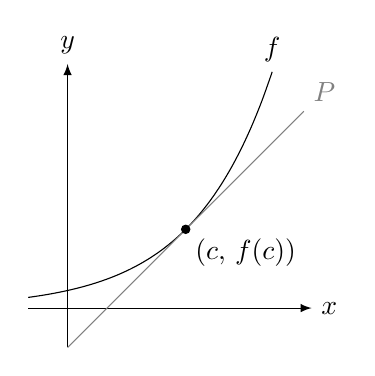
\begin{tikzpicture}
        \draw[-latex] (-.5,0)--(3.1,0) node[right]{$x$};
        \draw[-latex] (0,-.5)--(0,3.1) node[above] {$y$};
        \draw[] plot[smooth, domain=-.5:ln(3)+1.5] (\x, {e^(\x-1.5)}) node[anchor=south] {$f$};
        \draw[color=gray] plot[domain=0:3] (\x,{\x-.5}) node[anchor=south west] {$P$};
        \filldraw (1.5,1) circle (1.5pt) node[anchor=north west] {$(c,\,f(c))$};
        
    \end{tikzpicture}
\end{center}


The approximating polynomial is said to be \textbf{expanded about \textit{c}} or \textbf{centered at \textit{c}}. It should make sense that we require the slopes to match as there are an infinite number of polynomials that pass through $(c,\,f(c))$. This constraint, at the very least, makes the approximation look somewhat similar to $f$ at that point.\\
\\

\noindent\textbf{Introductory Example: First-Degree Polynomial Approximation of $\mathbf{f(x)=e^{x}}$: }\\
For the function $f(x)=e^x$, find a first degree polynomial function $P_1(x)=a_0+a_1 x$ whose value and slope agree with the value of the slope of $f$ at $x=0$.

\vspace{\stretch{1}}


    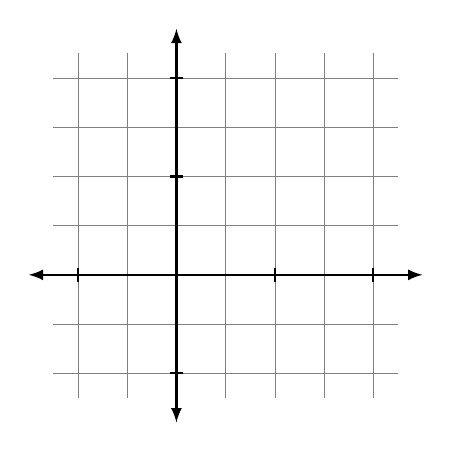
\begin{tikzpicture}[scale=1.25]
        \draw[style=help lines, step=.5] (-1.25,-1.25) grid (2.25,2.25);
        \draw[latex-latex,thick](-1.5,0)--(2.5,0);
        \draw[latex-latex,thick](0,-1.5)--(0,2.5);
        \foreach \x in {-1,1,2}
            \draw[thick] (\x,2pt)--(\x,-2pt);
        \foreach \y in {-1,1,2}
            \draw[thick] (2pt,\y)--(-2pt,\y);    
    \end{tikzpicture}


\newpage

Based on $P_1$ found in example 1, we can see that our approximation fits relatively well for values of $x$ that are close to $c=0$. However, the further we move away from $(0,1)$, it is clear that our approximation will not be accurate whatsoever. How might we improve the accuracy even further?\\

Let's consider the following:

\begin{minipage}{0.45\linewidth}
    \[P_2(x)=1+x+\frac{1}{2}x^2\]
\end{minipage}
\hfill
\begin{minipage}{0.45\linewidth}
    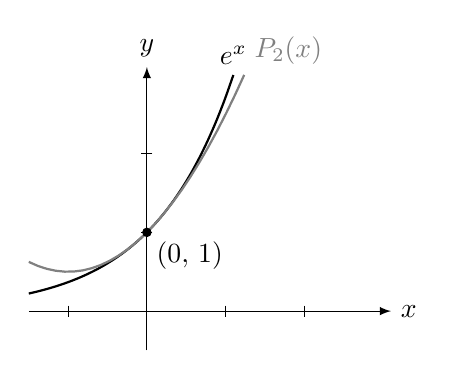
\begin{tikzpicture}
        \draw[-latex] (-1.5,0)--(3.1,0) node[right]{$x$};
        \draw[-latex] (0,-.5)--(0,3.1) node[above] {$y$};
        \foreach \x in {-1,1,2}
            \draw (\x,2pt)--(\x,-2pt);
        \foreach \y in {1,2}
            \draw (2pt,\y)--(-2pt,\y); 
        
        \draw[thick] plot[smooth, domain=-1.5:ln(3)] (\x, {e^(\x)}) node[anchor=south] {$e^x$};
        \draw[thick,color=gray] plot[domain=-1.5:1.236] (\x,{1+\x+.5*(\x)^2}) node[anchor=south west] {$P_2(x)$};
        \filldraw (0,1) circle (1.5pt) node[anchor=north west] {$(0,\,1)$};
        
    \end{tikzpicture}
\end{minipage}

\begin{minipage}{0.45\linewidth}
    \[P_3(x)=1+x+\frac{1}{2}x^2+\frac{1}{6}x^3\]
\end{minipage}
\hfill
\begin{minipage}{0.45\linewidth}
    \begin{tikzpicture}
        \draw[-latex] (-1.5,0)--(3.1,0) node[right]{$x$};
        \draw[-latex] (0,-.5)--(0,3.1) node[above] {$y$};
        \foreach \x in {-1,1,2}
            \draw (\x,2pt)--(\x,-2pt);
        \foreach \y in {1,2}
            \draw (2pt,\y)--(-2pt,\y); 
        
        \draw[thick] plot[smooth, domain=-1.5:ln(3)] (\x, {e^(\x)}) node[anchor=south east] {$e^x$};
        \draw[thick,color=gray] plot[domain=-1.5:1.125] (\x,{1+\x+.5*(\x)^2+1/6*(\x)^3}) node[anchor=south west] {$P_3(x)$};
        \filldraw (0,1) circle (1.5pt) node[anchor=north west] {$(0,\,1)$};
        
    \end{tikzpicture}
\end{minipage}

Clearly, $P_2$ is a better approximation than $P_1$, and $P_3$ more still. If we continue on, matching each $n$th derivative of $f(x)=e^x$ at $x=0$, we obtain the following:

\[P_n(x)=1+x+\frac{1}{2}x^2+\frac{1}{3!}x^3+\cdots+\frac{1}{n!}x^n\approx e^x\]

\vspace{.1in}

\begin{tcolorbox}[title= DEFINITIONS OF THE \textit{\textbf{n}}TH TAYLOR POLYNOMIAL AND \textbf{\textit{n}}TH MACLAURIN POLYNOMIAL,colframe=black,sharp corners,colback=white,colbacktitle=white,coltitle=black]

    If $f$ has $n$ derivatives at $c$, then the polynomial
    \[P_n(x)=f(c)+f'(c)(x-c)+\frac{f''(c)}{2!}(x-c)^2+\cdots+\frac{f^{(n)}(c)}{n!}(x-c)^n\]
    is called the \textbf{\textit{n}th Taylor Polynomial for \textit{f} at \textit{c}}. If $c=0$, then
    \[P_n(x)=f(0)+f'(0)(x)+\frac{f''(0)}{2!}x^2+\cdots+\frac{f^{(n)}(0)}{n!}x^n\]
    is also called the \textbf{\textit{n}th Maclaurin Polynomial for \textit{f}}. 

\end{tcolorbox}

\newpage

\noindent\textbf{Examples:}
\begin{questions}
    \question Find the $n$th Maclaurin polynomial for $f(x)=e^x$.
    \vspace{\stretch{1}}
    
    \question Find the Taylor polynomials $P_0,\,P_1,\,P_2,\,P_3,\,$and $P_4$ for $f(x)=\ln x$ centered at $c=1$.
    \vspace{\stretch{2.5}}
\end{questions}

\begin{minipage}{0.18\linewidth}
    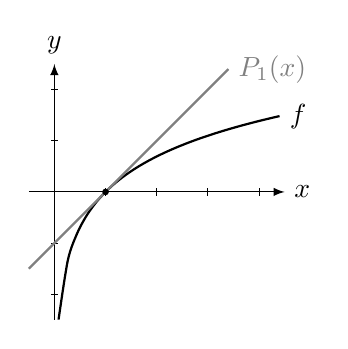
\begin{tikzpicture}[scale=.65]
        \draw[-latex] (-.5,0)--(4.5,0) node[right]{$x$};
        \draw[-latex] (0,-2.5)--(0,2.5) node[above] {$y$};
        \foreach \x in {1,2,3,4}
            \draw (\x,2pt)--(\x,-2pt);
        \foreach \y in {-2,-1,1,2}
            \draw (2pt,\y)--(-2pt,\y); 
        
        \draw[thick] plot[smooth, domain=e^(-2.5):4.4] (\x, {ln(\x)}) node[anchor=west] {$f$};
        \draw[thick,color=gray] plot[domain=-.5:3.4] (\x,{\x-1}) node[right] {$P_1(x)$};
        \filldraw (1,0) circle (1.5pt);
        
    \end{tikzpicture}
    \end{minipage}
    \hfill
    \begin{minipage}{0.18\linewidth}
        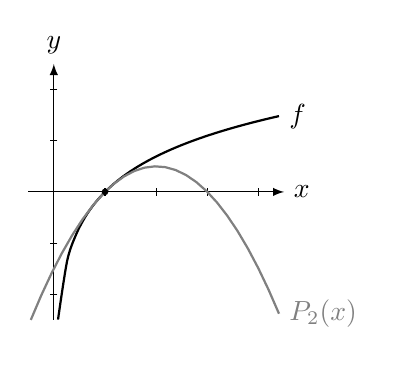
\begin{tikzpicture}[scale=.65]
            \draw[-latex] (-.5,0)--(4.5,0) node[right]{$x$};
            \draw[-latex] (0,-2.5)--(0,2.5) node[above] {$y$};
            \foreach \x in {1,2,3,4}
                \draw (\x,2pt)--(\x,-2pt);
            \foreach \y in {-2,-1,1,2}
                \draw (2pt,\y)--(-2pt,\y); 
            
            \draw[thick] plot[smooth, domain=e^(-2.5):4.4] (\x, {ln(\x)}) node[anchor=west] {$f$};
            \draw[thick,color=gray] plot[domain=-.45:4.4] (\x,{(\x-1)-1/2*(\x-1)^2}) node[right] {$P_2(x)$};
            \filldraw (1,0) circle (1.5pt);
            
        \end{tikzpicture}
    \end{minipage}
    \hfill
    \begin{minipage}{0.18\linewidth}
        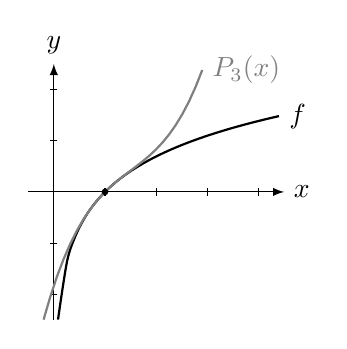
\begin{tikzpicture}[scale=.65]
            \draw[-latex] (-.5,0)--(4.5,0) node[right]{$x$};
            \draw[-latex] (0,-2.5)--(0,2.5) node[above] {$y$};
            \foreach \x in {1,2,3,4}
                \draw (\x,2pt)--(\x,-2pt);
            \foreach \y in {-2,-1,1,2}
                \draw (2pt,\y)--(-2pt,\y); 
            
            \draw[thick] plot[smooth, domain=e^(-2.5):4.4] (\x, {ln(\x)}) node[anchor=west] {$f$};
            \draw[thick,color=gray] plot[domain=-.2:2.9] (\x,{(\x-1)-1/2*(\x-1)^2+1/3*(\x-1)^3}) node[right] {$P_3(x)$};
            \filldraw (1,0) circle (1.5pt);
            
        \end{tikzpicture}
    \end{minipage}
    \hfill
    \begin{minipage}{0.18\linewidth}
        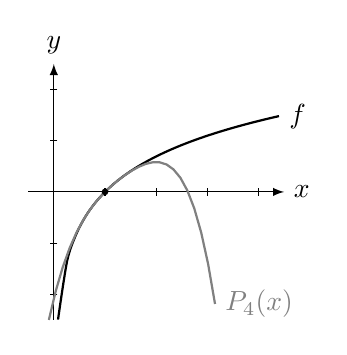
\begin{tikzpicture}[scale=.65]
            \draw[-latex] (-.5,0)--(4.5,0) node[right]{$x$};
            \draw[-latex] (0,-2.5)--(0,2.5) node[above] {$y$};
            \foreach \x in {1,2,3,4}
                \draw (\x,2pt)--(\x,-2pt);
            \foreach \y in {-2,-1,1,2}
                \draw (2pt,\y)--(-2pt,\y); 
            
            \draw[thick] plot[smooth, domain=e^(-2.5):4.4] (\x, {ln(\x)}) node[anchor=west] {$f$};
            \draw[thick,color=gray] plot[domain=-.097:3.15] (\x,{(\x-1)-1/2*(\x-1)^2+1/3*(\x-1)^3-1/4*(\x-1)^4}) node[right] {$P_4(x)$};
            \filldraw (1,0) circle (1.5pt);
            
        \end{tikzpicture}
    \end{minipage}
    
    \newpage


\begin{questions}
    \setcounter{question}{2}
    \question Find the Maclaurin Polynomials $P_n$ for $n=0,\,2,\,4,\,6$ for $f(x)=\cos x$. Then, use $P_6(x)$ to approximate the value of $\cos(0.1)$.
    \vspace{\stretch{1}}


    \question Find the third Taylor Polynomial for $f(x)=\sin x$, expanded about $c=\pi/6$.
    \vspace{\stretch{1}}

\end{questions}


\newpage
